\textbf{Causal networks} is the last notion that tell us something about the Bayesian networks, in particular it defines how to design networks that belong to an uncertain
domains. \vspace{3.5pt}

In the previous paragraph we saw that any ordering of nodes permits a consistent construction of the Bayesian network, but at the same time if the ordering respects the 
causality knowledge, the network seems to be easier to handle.
\begin{definition}
    \textbf{Causal networks} are a restricted class of Bayesian networks that forbids all but not causally compatible orderings.
\end{definition}
Let's clarify this concept with an example.
\begin{example}
    i.e. Assume this simple network, composed by two nodes. \vspace{3.5pt}
    \begin{center}
        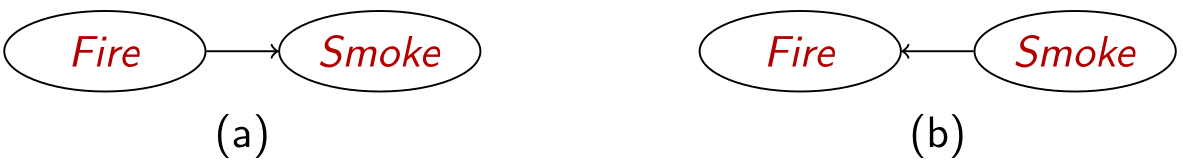
\includegraphics[width=0.65\textwidth]{img/img7.png}
    \end{center} \vspace{3.5pt}
    A and B represent the same domain and they are equally good distributions. Each of them produce the same full joint distribution, whatever the ordering of nodes chosen. 
    But these representation are not equivalent. Intuitively, the main difference is that the first graph follows \textbf{casuality}, instead the second one describes the
    diagnostic direction.
\end{example}
When defining causal networks we have to consider a particular question:
\begin{center}
    \textbf{which responds to which?}
\end{center}
It substitutes the initial question that we used to assume: \textit{is there any flow of influence?} 
We can define a recurrent method to answer the first question, as follows:
\begin{enumerate}
    \item Draw an arrow from \textbf{Fire} to \textbf{Smoke} if nature assigns a value to \textbf{Smoke} on the basis of what nature learns about \textbf{Fire}.
    \item Do not draw an arrow from \textbf{Smoke} to \textbf{Fire} if you judge that nature assigns a \textbf{Fire} a truth value based on variables other than \textbf{Smoke}.
    \item For each variable $X_i$ that can take values $x_i=f_i(OtherVariables)$, draw $X_j \rightarrow X_i$ iff $X_j$ is one of the arguments of $f_i$ 
    \begin{center}
        $x_i = f_i(\dots)$ is called \textbf{structural equation}
    \end{center}
\end{enumerate}
The last point might be a misunderstanding, it's simply defining which variables would be linked to $X_i$.
\begin{example}
    i.e. Lawn network. \vspace{3.5pt}
    \begin{center}
        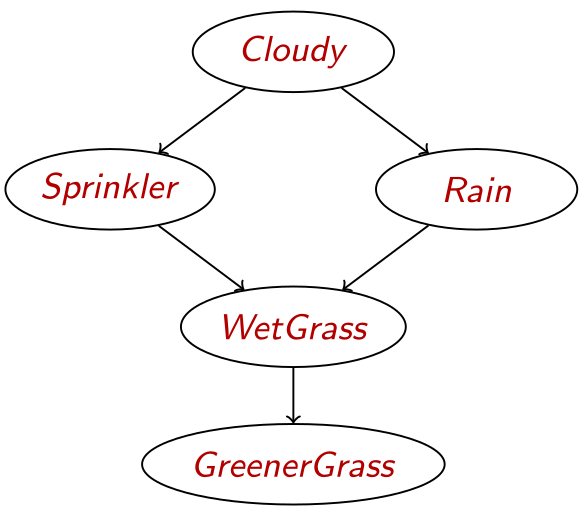
\includegraphics[width=0.4\textwidth]{img/img8.png}
    \end{center} \vspace{3.5pt}
    As written before, the data structure represents a Lawn network. It's possible to describe the same network by \textbf{structural equations}, as: \vspace{3.5pt}

    $C = f_C(U_C)$

    $R = f_R(C, U_R)$

    $S = f_S(C, U_S)$

    $W = f_W(S, R, U_W)$

    $G = f_G(W, U_G)$ \vspace{3.5pt}

    It's important to understand what structural equation semantic means. Generally $U_*$ stands for uncertainty, there are no nodes that are not dominated by \textbf{uncertainty}.
    Upper case letters, as $C$, $R$, $S$, $W$, $G$, define the nodes. Finally, $f_*(\dots)$ functions symbolise which random variables assign sample points to their child node; this is translated via a direct connection between nodes. \vspace{3.5pt}

    Furthermore, structural equations are capable to describe the same domain even if are made local changes in the environment. We assume that the sprinkler has been turned off. 
    The resulting representations via Bayesian network and structural equations change as: \vspace{3.5pt}
    \begin{center}
        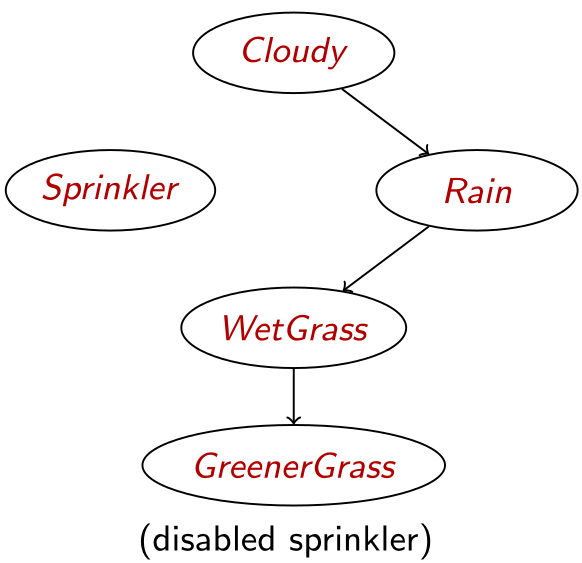
\includegraphics[width=0.4\textwidth]{img/img9.png}
    \end{center} \vspace{3.5pt}
    $C = f_C(U_C)$

    $R = f_R(C, U_R)$

    $S = f_S(U_S)$

    $W = f_W(R, U_W)$

    $G = f_G(W, U_G)$ \vspace{3.5pt}

    Again, if we cover the lawn such as Rain has not any effect, the representations are like: \vspace{3.5pt}
    \begin{center} 
        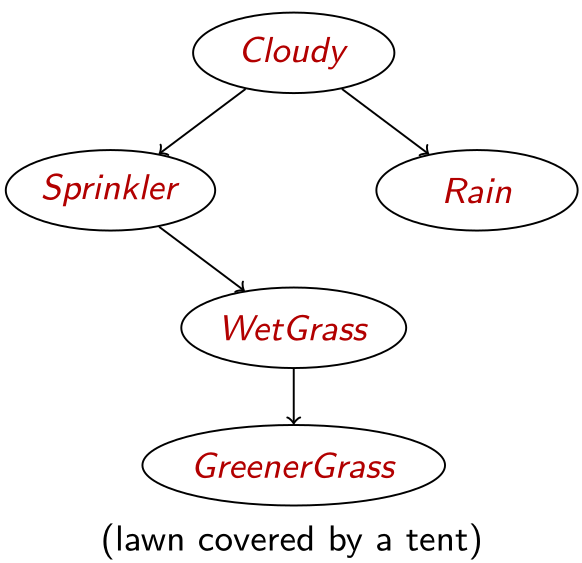
\includegraphics[width=0.4\textwidth]{img/img10.png}
    \end{center} \vspace{3.5pt}
    $C = f_C(U_C)$

    $R = f_R(C, U_R)$

    $S = f_S(C, U_S)$

    $W = f_W(S, U_W)$

    $G = f_G(W, U_G)$ \vspace{3.5pt}

    What happens if we set off Sprinkler? In probabilistic terms, it might be described as follows:
    \begin{center}
        $P(GreenerGrass|Sprinkler=True)$ = ?\footnote{Here, we are observing that Sprinkler is on.}
    \end{center} \vspace{3.5pt}

    This tricky question has two means: 
    \begin{itemize}
        \renewcommand{\labelitemi}{-}
        \item If Sprinkler is on, then the probability of WetGrass and GreenerGrass might increase.
        \item Sprinkler set off tell us that it's not raining outside. 
    \end{itemize} \vspace{3.5pt}

    These assertions gives a clue: we are expressing the same things as we might do with \textit{prior probabilities} and \textit{conditional probabilities}. However,
    the same changes are solved via Bayes nets semantics:
    \begin{center}
        $P(c, r, w, g|do(S = true))$\footnote{Instead, we are turning Sprinkler on to see what happens.}
    \end{center} \vspace{3.5pt}

    The right hand side of the argument is named \textbf{do-operator}. It allows to represent interventions and predict their observable consequences, without changing the domain.
\end{example}
Bayesian networks and structural equations express the domain exactly in the same way, but nevertheless there is a huge difference. If structural equations can afford interventions 
and domain still be the same, Bayesian network does not! In Bayesian networks we are deducing behavioral aspects observing some evidences, differently in structural equations 
we are deducing behavioral aspects doing some operations.